% !TEX program = xelatex
\documentclass[a4paper,14pt,oneside,openany]{memoir}

%%% Задаем поля, отступы и межстрочный интервал %%%

\usepackage[left=30mm, right=15mm, top=20mm, bottom=20mm]{geometry}
\pagestyle{plain}
\parindent=1.25cm
\usepackage{indentfirst}

%%% Задаем языковые параметры и шрифт %%%

\usepackage[english,russian]{babel}
\babelfont[russian]{rm}{Times New Roman}
\babelfont[russian]{tt}{Courier New}

%%% Задаем стиль заголовков и подзаголовков в тексте %%%

\setsecnumdepth{subsection}
\renewcommand*{\chapterheadstart}{}
\renewcommand*{\printchaptername}{}
\renewcommand*{\chapnumfont}{\normalfont\bfseries}
\renewcommand*{\afterchapternum}{\hspace{1em}}
\renewcommand*{\printchaptertitle}{\normalfont\bfseries\centering\MakeUppercase}
\setbeforesecskip{20pt}
\setaftersecskip{20pt}
\setsecheadstyle{\raggedright\normalfont\bfseries}
\setbeforesubsecskip{20pt}
\setaftersubsecskip{20pt}
\setsubsecheadstyle{\raggedright\normalfont\bfseries}

%%% Исправление нумерации секций %%%

\renewcommand{\thesection}{\arabic{section}}
\renewcommand{\thesubsection}{\arabic{subsection}}

%%% Сквозная нумерация рисунков и таблиц %%%

\counterwithout{figure}{chapter}
\counterwithout{table}{chapter}

%%% Выравнивание и переносы %%%

\tolerance 1414
\hbadness 1414
\emergencystretch 1.5em
\clubpenalty=10000
\widowpenalty=10000

%%% Задаем параметры оформления рисунков и таблиц %%%

\usepackage{graphicx}
\usepackage{caption}
\usepackage{subcaption}
\usepackage{float}
\graphicspath{{photo/}}
\captionsetup[figure]{font=small, width=\textwidth, name=Рисунок, justification=centering}
\captiondelim{ --- }
\usepackage[section]{placeins}

%%% Задаем параметры ссылок и гиперссылок %%% 

\usepackage{hyperref}
\hypersetup{
    colorlinks=true,
    linkcolor=red,
    citecolor=red
}

%%% Настраиваем отображение списков %%%

\usepackage{enumitem}
\renewcommand*{\labelitemi}{\normalfont{--}}
\setlist{noitemsep, leftmargin=*}

\begin{document}

% Титульный лист (без номера страницы)
\thispagestyle{empty}

\begin{center}
    МИНИСТЕРСТВО ЦИФРОВОГО РАЗВИТИЯ, СВЯЗИ И МАССОВЫХ \\ КОММУНИКАЦИЙ \\ РОССИЙСКОЙ ФЕДЕРАЦИИ

    \vspace{20pt}

    Федеральное государственное бюджетное образовательное учреждение \\ высшего образования \\
    "Сибирский государственный университет телекоммуникаций и \\ информатики"

    \vspace{20pt}

    Кафедра телекоммуникационных систем и вычислительных средств \\ (ТС и ВС)
\end{center}

\vfill

\begin{center}
    Практическая работа №10 \\
    по дисциплине \\
    \textit{"Web-технологии"}

    \vspace{20pt}

    по теме: \\
    \uppercase{Основы Figma}
\end{center}

\vfill

\noindent Студент: \\
\textit{Группа ИКС-532 \hfill А.С. Лёшин}

\vspace{20pt}

\noindent Преподаватель: \\
\textit{старший преподаватель \hfill А.В. Андреев}

\vfill

\begin{center}
    Новосибирск 2026 г.
\end{center}

\newpage
\setcounter{page}{2}
\OnehalfSpacing*

\subsection*{Цель работы}

\begin{itemize}
    \item Научиться создавать фрейм и работать с ним.
    \item Научиться работать с текстовыми слоями, геометрическими объектами, цветом и фото.
    \item Научиться настраивать Constraints (привязки).
    \item Научиться работать с Layout grid (сетка).
    \item Создать адаптивные версии макета для ПК, планшета и телефона.
\end{itemize}

\section{Введение}

В ходе выполнения данной практической работы производится разработка макета пользовательского интерфейса для интернет-магазина цветов и растений «Plant» с использованием облачного графического редактора Figma. Основное внимание уделяется проектированию десктопной версии сайта, подбору цветовой палитры, типографики, а также созданию удобной структуры каталога товаров и навигации. Дополнительно выполнены адаптивные версии для планшета (768px) и мобильного телефона (360px).

\section{Результаты выполнения}

Ниже представлены скриншоты разработанного макета интернет-магазина домашних растений для трёх устройств.

\subsection*{Версия для ПК (1440px)}
\begin{figure}[H]
    \centering
    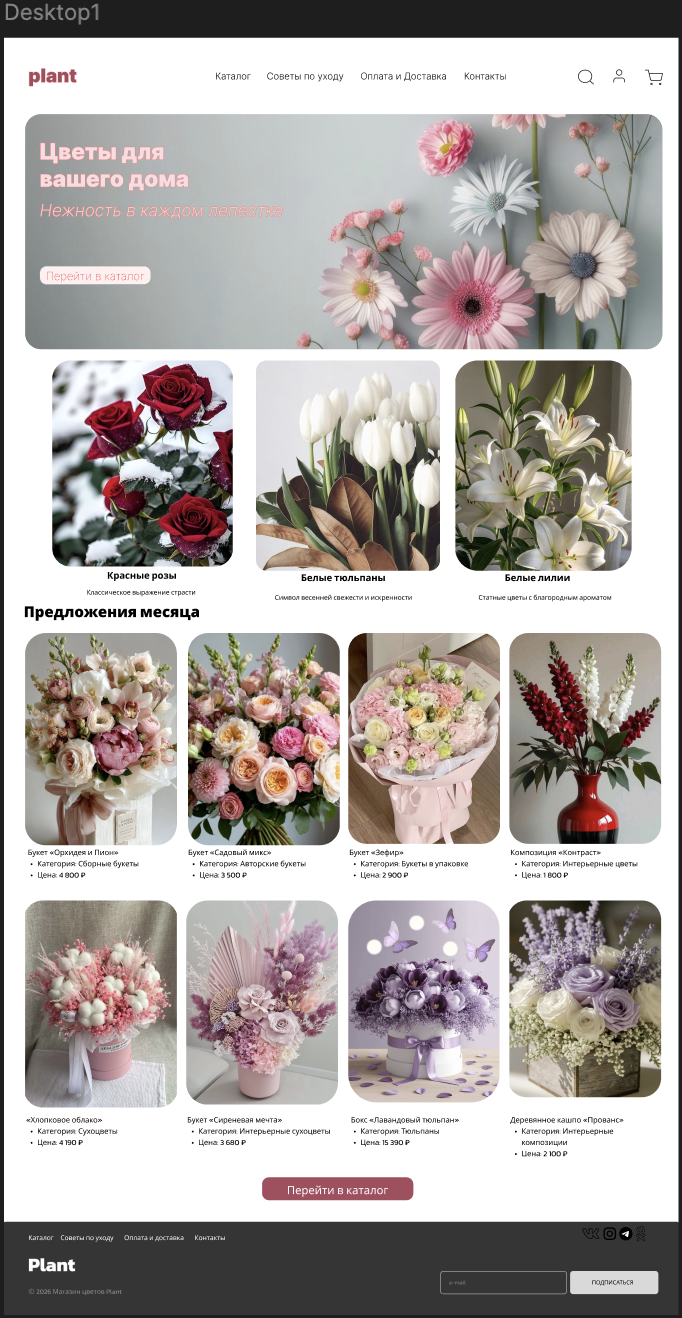
\includegraphics[width=0.7\textwidth]{photo/pc.png}
    \caption{Десктопная версия макета}
\end{figure}

\subsection*{Версия для планшета (768px)}
\begin{figure}[H]
    \centering
    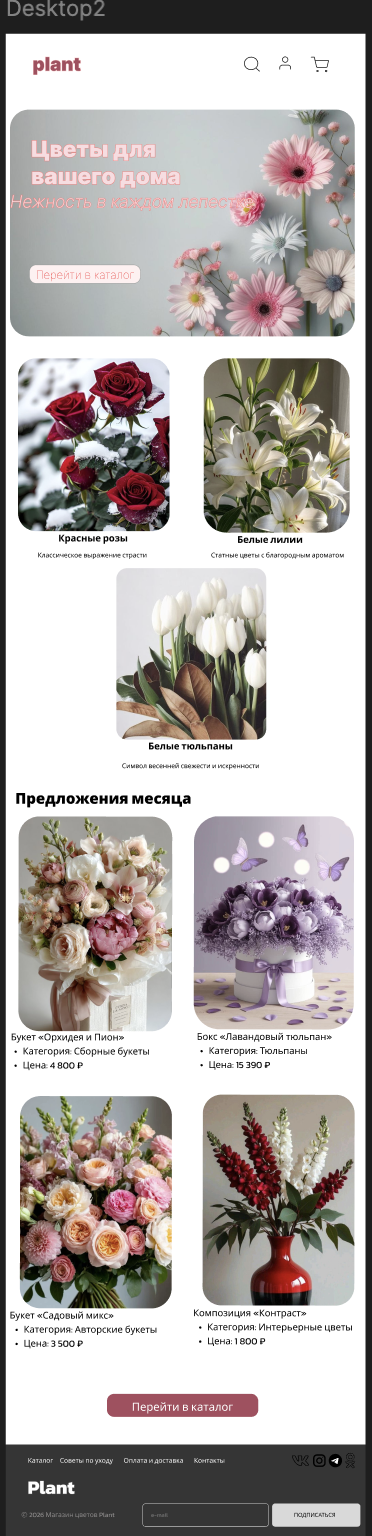
\includegraphics[width=0.3\textwidth]{photo/tablet.png}
    \caption{Адаптивная версия для планшета}
\end{figure}

\subsection*{Версия для мобильного телефона (360px)}
\begin{figure}[H]
    \centering
    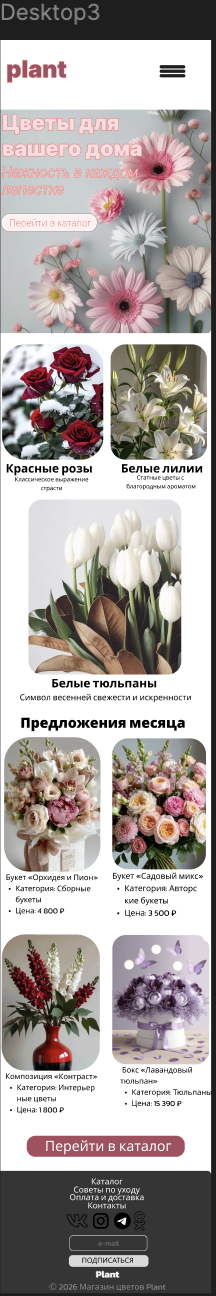
\includegraphics[width=0.2\textwidth]{photo/mobile.png}
    \caption{Адаптивная версия для мобильного телефона}
\end{figure}
\newpage
\subsection*{Ссылка на макет в Figma}

Работа доступна по ссылке: \\
\href{https://www.figma.com/design/1d8jKG7HBjWD7WZMPTWUL6/Untitled?node-id=0-1&p=f&t=tP8li9G6XxfsJLX0-0}{Макет интернет-магазина растений Plant}


\section*{Заключение}
\addcontentsline{toc}{section}{Заключение}

В ходе выполнения практической работы №10 были получены следующие результаты:
\begin{enumerate}
    \item Создан макет страницы интернет-магазина домашних растений.
    \item Реализованы шапка, меню, обложка с кнопкой, блок «Предложения месяца» и футер.
    \item Настроена колоночная сетка (Layout grid) и привязки (Constraints).
    \item Выполнены две адаптивные версии: 768px (планшет) и 360px (мобильный телефон).
    \item Макет опубликован в Figma и доступен по ссылке.
\end{enumerate}
\end{document}